\section{Analyse du projet} %cahier des charges

\subsection{Analyse de l'existant}

Plusieurs jeux au gameplay approchant celui visé par l’équipe ont été testés. Voici ce qu’il en ressort au niveau du gameplay.
\paragraph{Jeux basés sur la musique}
On y trouve souvent une musique par niveau. Il faut taper sur plusieurs notes en synchronisation avec la musique qui est jouée en arrière-plan. Les notes ont généralement été posées manuellement par les concepteurs, en fonction du niveau. Certains jeux permettent de charger directement ses propres MP3, la génération du niveau est donc faite à la volée en fonction du fichier.\\
\textit{Exemples : Guitar Hero sur console, TapTap sur iOS et applications de promotions d’album.}
\paragraph{Jeux basés sur l’habilité ryhtmique}
Il existe aussi des jeux basés sur l’habileté de l’utilisateur et sa vitesse de réaction où le principe est de taper sur l’écran au bon moment et au bon endroit. L'accent est mis sur le style graphique, il n'y a pas une grande variété dans les musiques et elles n'ont pas de lien direct avec les niveaux. La musique n'est là que pour apporter du rythme ainsi qu’un élément addictif, si elle est agréable à l’oreille.\\
\textit{Exemples : Geometry Dash, SineWave et Colorace sur smartphones.}
\paragraph{Jeu de type “Runner”}
Enfin, certains jeux ne proposent qu’un gameplay rapide et de beaux graphismes, en ne prêtant que peu d’importance à la musique. Le contenu du jeu est ainsi plus fourni en niveaux, en personnages et fonctionnalités et les graphismes du jeu sont donc, en conséquence, plus approfondis. L’utilisateur ne joue qu’en fonction de ce qui apparaît à l’écran. La musique peut changer en fonction de l’avancée dans le niveau.\\
\textit{Exemples : Temple Run sur mobile. Bit.Trip sur Wii et PC.}

\subsection{Cahier des charges}

\subsubsection{Principe de progression}
\paragraph{} Le joueur lance le jeu et découvre un monde totalement vide sans aucune animation ni effet sonore. Un simple métronome qui frappe la mesure retentit, et la mascotte, un escargot, se déplace en rythme sur cette planète de façon circulaire.
Le joueur doit débloquer des objets visuels et sonores dans des mini-jeux afin de rendre cette planète plus remplie et joyeuse.
\begin{center}
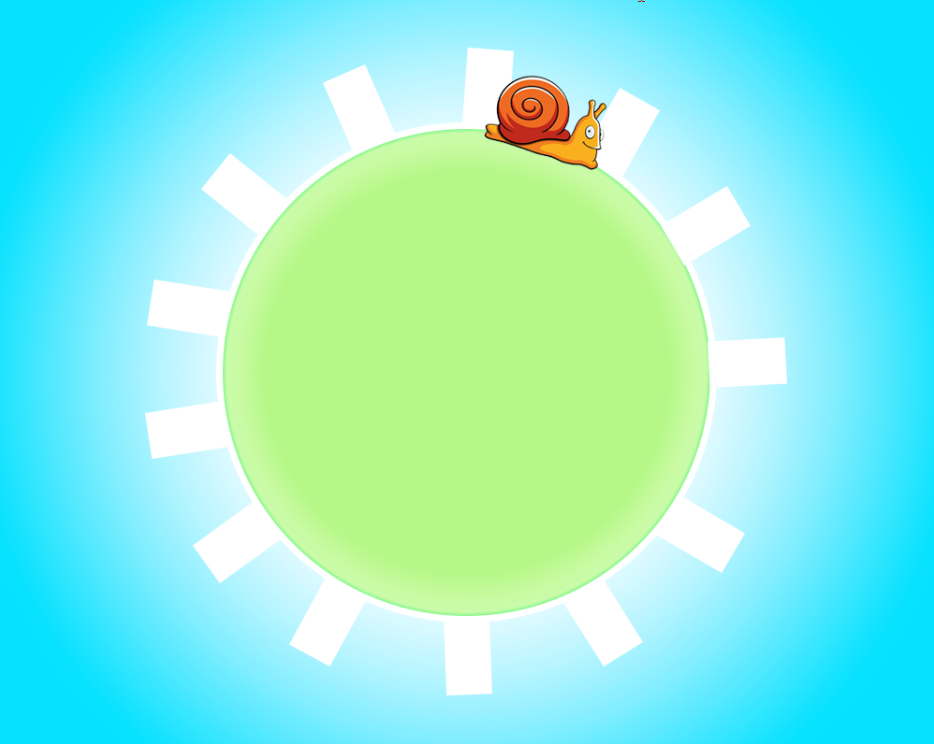
\includegraphics[scale=0.4]{img/protoPlanete.png}\\
\textit{Prototype de planète à remplir}
\end{center}
\paragraph{} Un objet est constitué d’un élément visuel qui est animé en rythme sur le tempo de la planète, et est associé à un sample unique qui est une composante d’une musique propre au jeu.\
\paragraph{}Ce sample peut être un kick, une basse, une mélodie... Le principe est de débloquer peu à peu chacun des éléments du morceau final. On compte entre 5 et 10 éléments (donc mini-jeux) pour compléter entièrement le morceau.
\paragraph{}Cette planète sert de représentation visuelle pour l’avancement du joueur.

\subsubsection{Concept de mini-jeu}
Un mini jeu est constitué d’une scène unique et minimaliste animée par une musique de fond entraînante.
\begin{center}
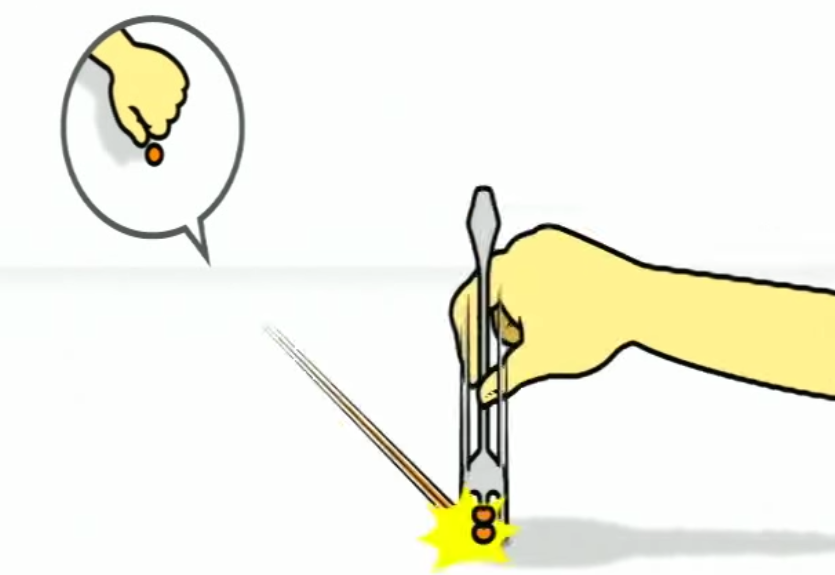
\includegraphics[scale=0.4]{img/rhythmParadise.png}\\
\textit{Exemple de mini jeu, présent dans le jeu "Rhythm Paradize"}
\end{center}
\paragraph{} Le joueur doit apprendre quelques mouvements propres au mini jeu dans un entraînement. Une fois les mouvements acquis, le joueur peut tenter de réussir le mini jeu. La musique commence, et il doit réussir un maximum de mouvements dans le temps fixé (1mn30 - 2mn environ)
\paragraph{} Ce mouvement peut être de nature varié : Il peut s’agir de tout simplement frapper un rythme synchronisé avec la musique, ou de répéter précisément une série de rythmes joués, ou de frapper après un signal avec un délai plus ou moins long, etc.
\paragraph{} A la fin du niveau, un score est généré. S’il est supérieur à un certain seuil exigé, le mini jeu passe en mode “réussi” et le joueur débloque l’objet associé sur sa planète.
Il existe plusieurs états pour un mini jeu :
\begin{itemize}
\item Non réalisé
\item Réussi
\item Super (Médaille)
\item Parfait
\end{itemize}
\paragraph{Notions techniques}
Les mini jeux sont uniques, c’est à dire qu’à chaque fois il s’agit d’un nouveau concept rythmique. Il n’est pas possible de les générer à la volée. On mettra en place des mécaniques précises qu’on pourra réutiliser sur chacun des mini jeux pour les créer le plus facilement possible. Pour les graphismes, de très simples dessins en 2D seront utilisés,. 

\subsubsection{Niveau infini}
\paragraph{} Une fois tous les éléments débloqués, le joueur atteint le niveau final qui est un mode infini arcade sur la musique assemblée dans lequel il peut essayer de réaliser le meilleur score possible en incarnant l’escargot. (Qui s’approche de notre idée de départ, mais de façon moins importante).

\paragraph{} La somme de ses scores réalisés au fil du temps est convertie sous la forme d’une monnaie avec laquelle il peut acheter des effets de lumières et décorations supplémentaires à disposer sur sa planète afin de la personnaliser.

\subsubsection{Partage}
L’avancement des joueurs, et la personnalisation des planètes, est stockée dans le cloud. Un joueur peut montrer sa planète à ses amis afin de montrer son avancement et ses scores.

\subsubsection{Monétisation}
En fonction de l’avancement final du projet, un système de monétisation sera choisi. Il pourra s’agir de la vente de monnaie supplémentaire pour la personnalisation par exemple.

\subsection{Objectifs du projet}

\paragraph{}
La liste des fonctionnalités à réaliser en fonction de leur importance pour un jeu jouable :
\begin{enumerate}
\item Réalisation de la planète animée et de ses éléments sonores (activables/désactivables)
\item Réalisation du moteur de mini-jeux rythmiques
\item Réalisation du mode de jeu infini/arcade
\\\\Puis :
\item Réalisation du système d’achat de lumières et de décorations supplémentaires avec la monnaie
\item Réalisation du système de partage in-cloud des planètes
\item Ajout d’autres planètes comprenant d’autres mini-jeux
\end{enumerate}

\subsection{Diagramme de Gantt prévisionnel}
\newpage
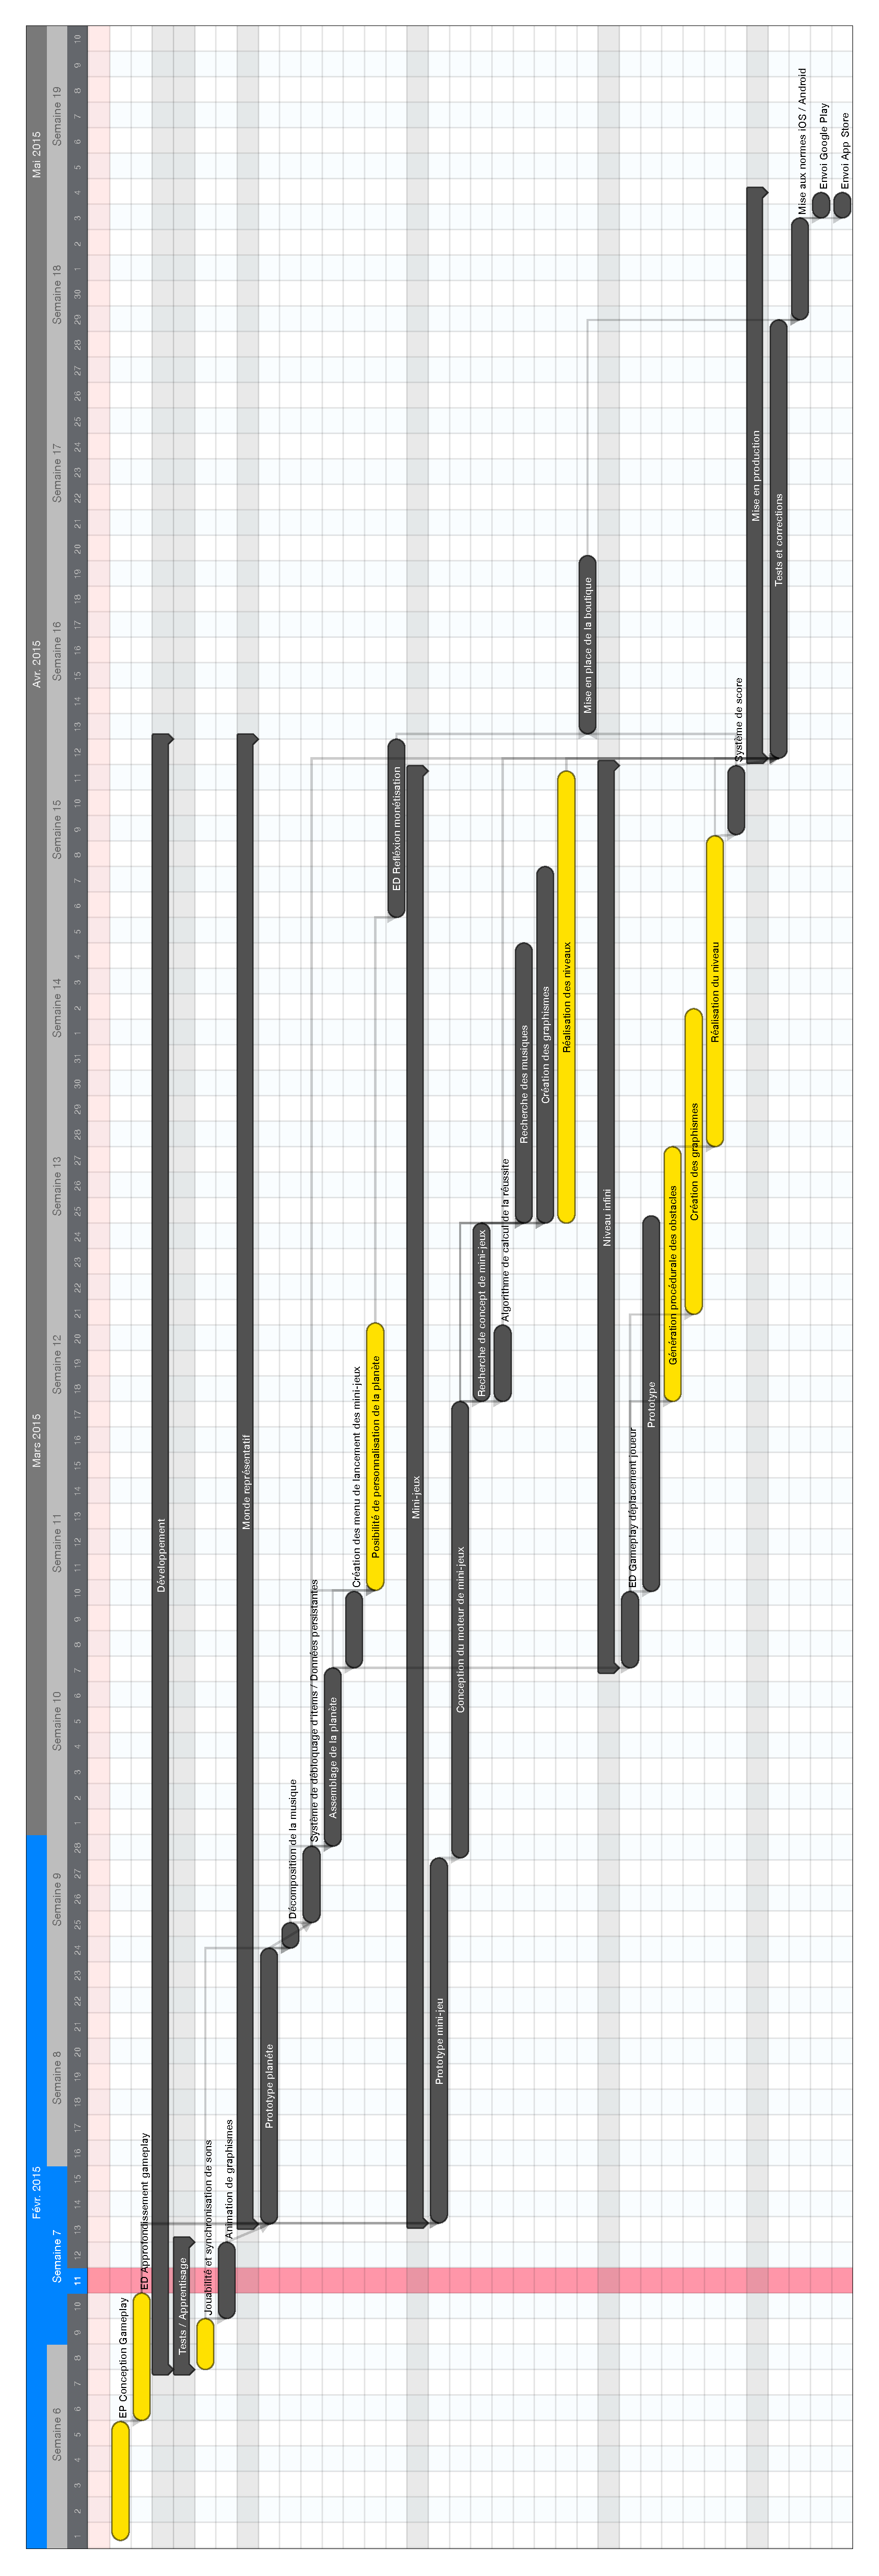
\includepdf{./feuilleDeRoute/oufGantt3.pdf}
